As was discussed in Section~\ref{subsec:structure}, the vast majority of our
attributes will not be considered at this stage of our analysis so we can focus
on how the cost of care is distributed and seen in the data. The exclusion of
these attributes does not, however, imply that they are not of interest. In
fact, when we look at the distributions of our subset of attributes on the whole
dataset we see that the data is skewed towards low-cost, short-stay, and
otherwise low-impact patients with long, heavy tails, as seen in
Figures~\ref{fig:netcost_kde}~\--~\ref{fig:no_proc_hist}. Then we can take
advantage of these other attributes, incorporating combinations of their values
to identify slices of the dataset which are of interest to our research.

\graphicspath{{./img/general/}}

\begin{figure}[h]
    \centering
    \begin{minipage}{.5\textwidth}
        \centering
        \includegraphics[width=.9\linewidth]{netcost_kde/main.pdf}
        \captionof{figure}{Estimated probability density for the net cost of a
        spell, clipped at \pounds12,500.}\label{fig:netcost_kde}
    \end{minipage}%
    \begin{minipage}{.5\textwidth}
        \centering
        \includegraphics[width=.9\linewidth]{los_hist/main.pdf}
        \captionof{figure}{Histogram for the total length of a spell, clipped
        at 21 days.}\label{fig:los_hist}
    \end{minipage}

    \begin{minipage}{.5\textwidth}
        \centering
        \includegraphics[width=.9\linewidth]{no_diag_hist/main.pdf}
        \captionof{figure}{Histogram for the number of diagnoses in an
        episode}\label{fig:no_diag_hist}
    \end{minipage}%
    \begin{minipage}{.5\textwidth}
        \centering
        \includegraphics[width=.9\linewidth]{no_proc_hist/main.pdf}
        \captionof{figure}{Histogram for the number of procedures in an
        episode}\label{fig:no_proc_hist}
    \end{minipage}
\end{figure}

There are many methods available to attempt tackling this skewedness including
the scaling and transformation of our attributes, but that is not to say that
all the attributes are so harshly skewed; Figure~\ref{fig:age_hist} shows the
clear peaks and troughs in the distribution of the ages of our patients.

\begin{figure}[h]
    \centering
    \includegraphics[width=.5\linewidth]{age_hist/main.pdf}
    \caption{Histogram for the age of patients with two-year
    bins.}\label{fig:age_hist}
\end{figure}
